\documentclass[main.tex]{subfiles}
\begin{document}
	
	% TODO: extensions are module specific, various extensions, coprehensive understanding, purpose of following sections 
	
	The various extensions of the Glasgow Haskell Compiler can be overwhelming at first. Understanding every single one of them requires a comprehensive knowledge of the compiler's countless features. This chapter aims at giving a general overview of the different kinds of extensions GHC provides.
	
	Different compilers can support different language extensions. Throughout the rest of this chapter, we will discuss the extensions provided by the Glasgow Haskell Compiler, the most widely used Haskell compiler. GHC implements a daunting number of 110 extensions. It would be difficult to deal with every single language extension, so we will consider only those that are used in more than one thousand modules throughout the Hackage database \cite{hackage-bib}, and those that are closely related to them. We measured the number of occurrences of each extension in the Hackage database, and collected the most popular ones. Their relative occurrences can be seen in Diagram~\ref{fig:rel-ext-piechart}. For the list of extensions in each category and their exact number of occurrences see Tables~(\ref{table:syn-exts-stats})--(\ref{table:other-exts-stats}).
	
	\begin{figure}[h]
		\renewcommand{\figurename}{Diagram}
		\hspace{-1cm}
		\centering
		\caption{Relative extension usage statistics}
		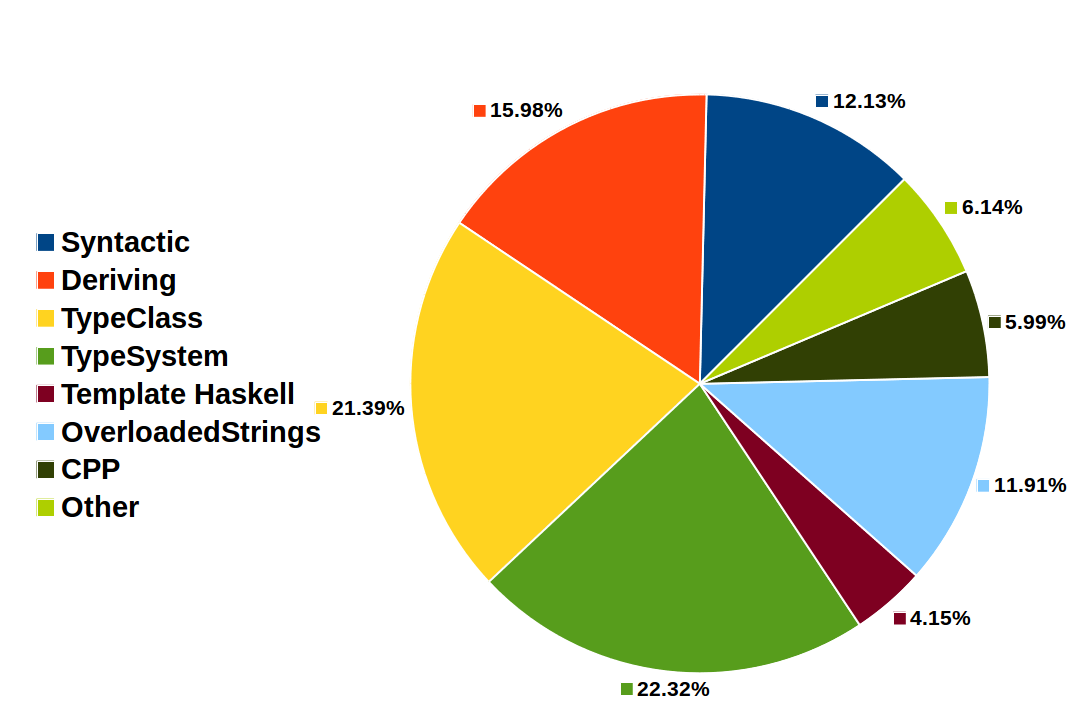
\includegraphics[scale=0.5]{extension_categories_pie}
		\label{fig:rel-ext-piechart}
	\end{figure}
	
	\section{Extension categories based on functionality} \label{extension-categories}
	
	We found over 30 extensions that are relevant enough to examine. Each of these extensions are present in more than one thousand modules in the Hackage database, and together they cover more than 90\% of the total occurrences of all extensions. In this section we will categorize these extensions based on their functionality. We will distinguish eight distinct groups. Within each group, one or two extensions will be presented in order to illustrate the functionalities of the extensions residing in those categories.
	
	Two groups contain only a single extension. These two groups are \ext{CPP} and \ext{OverloadedStrings}. They are quite unique extensions on their own, and are used often enough so that they will be discussed separately.
	
	\subsection{Syntactic extensions} \label{syntactic-exts}
	
	The Syntactic group consists of extension that either modify some part of the grammar of Haskell (e.g.: \ext{TypeOperators} allows operator names to be used as type identifiers), or they enrich the language with syntactic sugar. Syntactic sugar provide alternative ways to express already existing language constructs, thus making the language "sweeter" for human use. 
	
	The most significant extension in this category is \ext{RecordWildcards}, which enables wildcard pattern patching on record fields. Using \ext{RecordWildcards}, we do not have to specify the exact names of the fields when pattern matching: the wildcard pattern will match the set of all fields of the record. Hence, adding a new field to a record type will not affect our patterns. This feature can be exceptionally useful if we want to make our code forward-compatible with future changes.
	
	\begin{table}[h]
		\centering
		\rowcolors{2}{gray!25}{white}
		\caption{Usage statistics of syntactic extensions}
		\begin{tabular}{ | l r | }
			\hline
			\rowcolor{gray!50}
			Extension	& No. occurrences \\
			\hline
			\ext{RecordWildCards} & 8543 \\
			\ext{TypeOperators} & 5179 \\
			\ext{TupleSections} & 1792 \\
			\ext{LambdaCase} & 1357 \\
			\ext{ViewPatterns} & 1147 \\
			\ext{MagicHash} & 1115 \\
			\ext{MultiWayIf} & 248 \\
			\ext{ParallelListComp} & 161 \\
			\ext{GADTSyntax} & 9 \\
			\hline
		\end{tabular}
		\label{table:syn-exts-stats}
	\end{table}
	
	\subsection{Extensions to the type system} \label{type-system-exts}
	
	Haskell has a rich type system, providing a plethora of useful features such as type classes, parametric polymorphism and higher order functions. However, many of these features have certain limitations. Fortunately, the Glasgow Haskell Compiler presents some solutions in the form of language extensions, that lift these limitations. 
	
	Despite the advanced type system of Haskell, programmers often utilize language constructs that require a type system related extension. In fact, these extensions are the most frequently used ones. As we can see on Diagram~\ref{fig:rel-ext-piechart}, extensions to the type system and the type class system contribute more than 40\% to the total number of extensions used across all Haskell modules.
	
	This phenomenon can be explained by examining the extensions residing in these groups. Those that are not type class related, usually bring whole new constructs into language. These new elements can substantially enhance the programming experience, and often there are no standard compliant alternatives in the language. Hence, programmers tend to turn on an extension or two to ease software development.
	
	\ext{TypeFamilies} is the most notable member of this group, it alone has a higher than 5\% share of used extensions. \ext{TypeFamilies} introduces type-indexed data types and functions over types to the language~\cite{type-families}. These two features together enable type level programming and are useful for defining highly parameterized library interfaces. For instance, Haskell Tools uses \ext{TypeFamilies} to differentiate the semantic information present in nodes at different stages of the syntax tree construction. The extension allows us to define a mapping between the stages of construction and the types of semantic information. This way we can specify a highly parameterized representation of the abstract syntax tree.
	
	\begin{table}[h]
		\centering
		\rowcolors{2}{gray!25}{white}
		\caption{Usage statistics of type system related extensions}
		\begin{tabular}{ | l r | }
			\hline
			\rowcolor{gray!50}
			Extension	& No. occurrences \\
			\hline
			\ext{TypeFamilies} & 10859 \\
			\ext{ScopedTypeVariables} &	8156 \\
			\ext{DataKinds}	& 4989 \\
			\ext{RankNTypes} & 3092 \\
			\ext{GADTs} & 2938 \\
			\ext{ConstraintKinds}	& 2369 \\
			\ext{KindSignatures} & 2223 \\
			\ext{ExistentialQuantification}	& 1320 \\
			\ext{TypeFamilyDependencies} & 25 \\
			\hline
		\end{tabular}
		\label{table:type-system-exts-stats}
	\end{table}
	
	\subsection{Type class related extensions}
	
	As mentioned earlier, GHC's type system related extensions are the most commonly used ones. One group of extensions in this category is the group of type class related extensions.
	
	Type classes introduce a new feature to the type system, called \emph{ad hoc polymorphism}, often referred to as \emph{overloading}. In Haskell, types can have constraints that enforce limitations on the possible type variables the type can be instantiated with. These constraints are usually called the \emph{context} of the type. Ad hoc polymorphic expressions can have different meaning based on their context, more precisely, their semantics depend on the type variables they are instantiated with. A well-known example is the \ilcode{(==)} operator that has different meaning based on the type of its operands.
	
	Each type class defines an interface, all of its instances must obey this interface. We say that a type is an instance of a type class if it implements a minimally required set of functions specified by the type class. For example, all instances of the class \ilcode{Eq} have functions \ilcode{(==)} and \ilcode{(/=)} defined over them, but implementing only one of them is sufficient, since both of them can be mutually defined in terms of the other, as shown in Program~code~\ref{code:minimal-instance}.
	
	\vspace{-1cm}
	\noindent
	\begin{codeFloat}
		\begin{minipage}{0.47\textwidth}
			\begin{haskell}
				class Eq a where
				(==) :: a -> a -> Bool
				(==) x y = not (x /= y)
				
				(/=) :: a -> a -> Bool
				(/=) x y = not (x == y)
			\end{haskell}
		\end{minipage}
		\hfill
		\begin{minipage}{0.51\textwidth}
			\begin{haskell}
				instance Eq (Maybe a) where
				(==) (Just x) (Just y) = x == y
				(==) Nothing  Nothing  = True
				(==) _        _        = False
				
				-- defining (/=) is not needed	  
			\end{haskell}
		\end{minipage}
		\caption{Minimal instance example}
		\label{code:minimal-instance}
	\end{codeFloat}
	
	Despite the wide variety of features type classes bring into the language, they have their limitations. The usage of type classes is heavily restricted in GHC in order to ensure the type checking terminates faster and more safely. In practice, these limitations are overly restricting, and they can be lifted using certain language extensions~\cite{type-classes}. In particular, three restrictions regularly arise when programming is Haskell. The first one of these is that type classes can only be parameterized with a single type variable. This restriction can be lifted by turning on \ext{MultiParamTypeClasses}, which lets us define type classes with multiple type variables. The other two limitations are that class constraints and class instances must be simple (for more information see Sections~\ref{flexible-contexts}). These can be lifted by turning on \ext{FlexibleContexts} and \ext{FlexibleInstances} respectively.
	
	\begin{table}[h]
		\centering
		\rowcolors{2}{gray!25}{white}
		\caption{Usage statistics of type class related extensions}
		\begin{tabular}{ | l r | }
			\hline
			\rowcolor{gray!50}
			Extension	& No. occurrences \\
			\hline
			\ext{FlexibleInstances} & 11534 \\
			\ext{FlexibleContexts} & 8109 \\
			\ext{MultiParamTypeClasses} & 7361 \\
			\ext{UndecidableInstances} & 3126 \\
			\ext{TypeSynonymInstances} & 2736 \\
			\ext{FunctionalDependencies} & 1191 \\
			\ext{DefaultSignatures} & 388 \\
			\ext{ConstrainedClassMethods} & 22 \\
			\hline
		\end{tabular}
		\label{table:type-class-exts-stats}
	\end{table}
	
	\subsection{Extensions to the deriving mechanism}
	
	In Haskell, and in many other programming languages too, when we define our own data types, we usually want to perform certain operations on them. The most commonly known examples are the equality comparison (\ilcode{Eq}), the printing/parsing (\ilcode{Show}/\ilcode{Read}) functions or the uniform function application (\ilcode{Functor}). By default, these functions are not defined for our custom data types, so we have to manually instantiate the corresponding type classes. In the case of a complex data structure, this can result in writing several lines of boiler plate code, despite the implementation of these instances being trivial. These code segments are insignificant from the perspective of the business logic and only clutter our modules.
	
	Fortunately, GHC provides the deriving mechanism, which allows programmers to attach so-called deriving clauses to their data type declarations. In these deriving clauses we can specify certain type classes that will be automatically instantiated with our custom data type. This mechanism only permits the derivation of some predefined type classes, including, but not limited to \ilcode{Eq}, \ilcode{Ord}, \ilcode{Enum}, \ilcode{Functor}, \ilcode{Traversable} etc.
	
	In order to derive a class instance for our type, we must make sure it satisfies some conditions stated by the deriving algorithm for the class. This is necessary because in some cases automatic derivation of type class instances for our type might not be feasible. For example, GHC cannot generate \ilcode{Eq} instances for function types. Which makes sense, because deciding extensional equality of functions is considered computationally unmanageable.
	
	As of GHC 8.2.1 we can not only specify the type class we want to derive for our type, but the method of the deriving as well by using \ext{DerivingStrategies}. For instance, we can ask the compiler to utilize the default method definitions of the type class, instead of deriving them. This can be useful if the class in question has an empty minimal set, which means we do not have to define any class methods to instantiate it for our type. This feature is mostly used in generic programming in conjunction with other extensions such as \ext{DeriveGeneric} and \ext{DefaultSignatures}.
	
	\begin{table}[h]
		\centering
		\rowcolors{2}{gray!25}{white}
		\caption{Usage statistics of deriving extensions}
		\begin{tabular}{ | l r | }
			\hline
			\rowcolor{gray!50}
			Extension	& No. occurrences \\
			\hline
			\ext{DeriveDataTypeable} & 11208 \\
			\ext{DeriveGeneric} & 8068 \\
			\ext{DeriveFunctor} & 1037 \\
			\ext{DeriveFoldable} & 386 \\
			\ext{DeriveTraversable} & 384 \\
			\ext{DeriveAnyClass} & 244 \\
			\ext{DeriveLift} & 3 \\
			\ext{GeneralizedNewtypeDeriving} & 3318 \\
			\ext{StandaloneDeriving} & 1108 \\
			\hline
		\end{tabular}
		\label{table:deriv-exts-stats}
	\end{table}
	
	\subsection{Template Haskell} \label{template-haskell}
	
	\ext{TemplateHaskell} \cite{template-haskell-bib} brings compile-time meta-programming into Haskell. This essentially means that we can generate code in our modules based on compile-time decisions. Furthermore, this family of extensions not only allows for generating code, but also for converting Haskell syntax into Template Haskell representation. These conversions can be done using the splice and oxford brackets respectively. The former is called \emph{splicing}, the latter is called \emph{quoting}. \ext{TemplateHaskell} can be used as a code generator to avoid writing many lines of boilerplate code such as the instantiation of user-defined type classes for certain types. As a concrete example, Haskell-Tools uses the extension to generate data-accessors, called references~\cite{references-bib} for its AST nodes.
	
	There is a type of quoting which is worth mentioning, called quasi-quoting \cite{quasi-quote-bib}. Quasi-quoting makes it possible to define custom parsers for converting Haskell syntax into the Template Haskell representation. Quasi-quoters make the embedding of domain specific languages into the Haskell host language much easier. 
	
	One interesting property of \ext{TemplateHaskell} is that it requires multiple iterations of compilation, which can significantly increase the compilation time of a module. Moreover, using \ext{TemplateHaskell} can pose problems for static code analyzer tools, since the code segment generated by a splice can be different each time we compile the module. This means, the analyzing tool will only see one of the many possible syntax trees.
	
	\begin{table}[h]
		\centering
		\rowcolors{2}{gray!25}{white}
		\caption{Usage statistics of Template Haskell extensions}
		\begin{tabular}{ | l r | }
			\hline
			\rowcolor{gray!50}
			Extension	& No. occurrences \\
			\hline
			\ext{TemplateHaskell} & 5443 \\
			\ext{QuasiQuotes} & 1221 \\
			\ext{TemplateHaskellQuotes} & 26 \\
			\hline
		\end{tabular}
		\label{table:th-exts-stats}
	\end{table}
	
	\subsection{C preprocessor}
	
	Most programmers encounter with the C preprocessor when they learn \ext{C} or \ext{C++}. It is a less known fact that Haskell also supports the very same preprocessor as those two languages. The \ext{CPP} language extension enables using preprocessor directives and macros in Haskell modules. Probably the most important feature of the preprocessor is conditional compilation, which allows for compiling different code segments based on certain conditions. For instance, we can execute different pieces of code based on the operating system our application runs on. Another notable example is when writing robust libraries, we usually want to support many distinct versions of the same compiler; however, different variants can have different standard libraries, or distinctive language features. Using incompatible versions may result in compilation errors. Issues similar to these can be easily resolved by introducing conditionally compiled code into our modules based on the version number of the compiler in question. Hence, we can use the most recent language standard throughout our whole library, while still supporting older variants by writing a few extra lines of code (e.g.: including some additional imports, or turning on certain extensions).
	
	Just like with many other great features, using \ext{CPP} comes at a cost. As we mentioned in section~\ref{template-haskell}, changing the source code of a module at compile time can result in many distinctive syntax trees. In the case of using conditional compilation, GHC can only see one particular version of the code after preprocessing, which means, that any analysis done on the syntax tree generated from that code will be incomplete. It is worth noting that alongside with \ext{TemplateHaskell}, \ext{CPP} is the only extension that can affect our code at compile time.
	
	\subsection{Overloaded Strings} \label{overloaded-strings}
	
	For functional languages (Haskell in particular), the basic data structure of choice is the linked list. The main reason for this is that linked lists are the simplest recursive data structure. In Haskell, even plain strings are represented with lists of characters. This can come really handy for beginner Haskell programmers, since they can immediately start working with strings, right after they learned the basics of lists. For this very reason, GHC introduces syntactic sugar for string literals. It will automatically convert any series of characters between quotation marks into a list containing those characters. So the \ilcode{"abc"} string literal is the same thing as \ilcode{['a','b','c']}.
	
	However, linked lists can perform quite poorly in many situations, due to the many indirections caused by the pointers linking the elements together. Fortunately, many efficient string representations exist, such as \ilcode{FastString}, \ilcode{ByteString} or the most commonly used one: \ilcode{Text}. All of these implementations are unique on their own, and each serve a different purpose. For example, \ilcode{ByteString} can very efficiently handle binary data, but does not support UNICODE characters as \ilcode{Text} does.
	
	Despite these highly-performing implementations, a string literal will still mean a simple linked list of characters. \ext{OverloadedStrings} solves this problem by introducing context sensitive types for string literals: the very same literal can have different types based on the context of its occurrence. Basically, what GHC does is that instead of typing every single string literal as \ilcode{[Char]}, it will give them the type \ilcode{IsString a => a}. The \ilcode{IsString} type class is responsible for converting expressions of type \ilcode{[Char]} to our custom representation. Also, when pattern matching occurs on an overloaded string literal, the input argument is compared against the representation generated from the literal by \ilcode{IsString}, using standard equality comparison.
	
	It is also worth mentioning that a feature like this already exists in GHC for numeric literals. The very same idea is used there as well to overload numeric literals with the \ilcode{Num} and \ilcode{Fractional} type classes. The former is used for whole numbers, the latter is used for rational numbers. Both of these features really only introduce syntactic sugar to the language, but \ext{OverloadedStrings} is such a prevalent language extension it deserves to be discussed separately.  
	
	% can be implemented by modifying only the syntactic phase of compilation
	
	\subsection{Other extensions}
	
	There are some extensions in GHC which could not really fit into any of the categories above. The two most important ones among them are \ext{BangPatterns} and \ext{PatternSynonyms}.
	
	By default, Haskell is a lazy language, which basically means a value is calculated when it is needed. Until that point, values are stored as \emph{thunks}. Thunks can be regarded as unevaluated expressions. Whenever the value of a thunk is a needed, it will be calculated. At least to a certain extent. If only the first three elements of a list are needed, then only the first three elements will be computed. Sometimes it is desirable to control the laziness of the language to avoid the accumulation of thunks in order to prevent memory overuse. By using \ext{BangPatterns}, we can explicitly ask the compiler to strictly evaluate certain parts of a pattern. This feature is really useful when working with lots of numerical data.
	
	Haskell provides abstraction over many different language elements. Patterns are an exception. \ext{PatternSynonyms} resolves this issue by making patterns first class elements of the language. This means, it allows for the declaration of user-defined patterns.
	
	In Table~\ref{table:other-exts-stats}, we summarized the usage statistics of extensions in this category. The statistics of \ext{OverloadedStrings} and \ext{CPP} can also be found in this table.
	
	\begin{table}[h]
		\centering
		\rowcolors{2}{gray!25}{white}
		\caption{Usage statistics of \ext{CPP}, \ext{OverloadedStrings} and other extensions}
		\begin{tabular}{ | l r | }
			\hline
			\rowcolor{gray!50}
			Extension	& No. occurrences \\
			\hline
			\ext{OverloadedStrings} & 19187 \\
			\ext{CPP} & 9652 \\
			\ext{BangPatterns} & 3375 \\
			\ext{PatternSynonyms} & 2826 \\
			\ext{ForeignFunctionInterface} & 1850 \\
			\ext{ImplicitParams} & 1361 \\
			\ext{UnboxedTuples} & 481 \\
			\hline
		\end{tabular}
		\label{table:other-exts-stats}
	\end{table} 
		
	\section{Implication relations} \label{relations-of-extensions}
	
	By defining such a wide range of many different extensions, some relations naturally form between certain extensions. The language extensions supported by GHC have so-called \emph{implication relations} defined over them. Extension \textbf{A} \emph{implies} extension \textbf{B} if and only if turning on \textbf{A} requires turning on \textbf{B}. These implication relations are implicit, which means turning on an extension implicitly turns on all corresponding implied extensions. For instance, if we use \ext{GADTs} in our module, then (besides others extensions) \ext{GADTSyntax} is automatically turned on for us, we do not have to turn it on manually. It is also worth mentioning, that the implication relation is transitive.
	
	The complete network of implication relations among the extensions supported by GHC can be represented by a group of directed acyclic graphs, as shown in Figures~(\ref{fig:explicit-namespaces-dag})--(\ref{fig:others-dag}). In these graphs only the immediate implications are illustrated, transitive ones are not.
	
	The implication relations play a crucial role from the perspective of extension elimination. In order to remove a certain extension from a module, we must be able to determine if the extension is necessary. We can achieve this by analyzing the syntax tree of the module, and finding all the language elements requiring the given extension. If we did not find any language elements, we can safely remove the extension.	We define so-called \emph{checkers} for each individual extension, which are responsible for finding the language elements requiring the corresponding extension. If extension \textbf{A} implies extensions \textbf{B} and \textbf{C}, after eliminating \textbf{A}, we must explicitly turn on \textbf{B} and \textbf{C}, because the module might still use the functionalities provided by the latter two. If we want to completely remove \textbf{A}, we must define checkers for the other two extensions as well. Unfortunately, in some cases this is not possible.
	
	%\subfile{extension_relations_forest}
	
	
\end{document}